\section{Cross team process}
The definition of the development process of \gls{G19} resulted in a manual\cite{processManual} written by the \gls{SMT}. The manual defines the practices and process we agreed should be followed by the \glspl{devTeam}. The previously mentioned manual contains all the decisions in the following sections.

The GIRAF coordinator arranged a presentation by Anton Christensen, a student of \gls{G18}. Christensen described how his year had worked in teams that focused on one part of the system. He described that this way of dividing the work made the developers very dependent on each other, and this had been an issue for the groups. We decided to use another method, where the teams are \Glspl{fullStack}, which means, that the teams work on the complete vertical slice of a user story rather than just on a single layer.
\begin{figure}[H]
        \begin{center}
            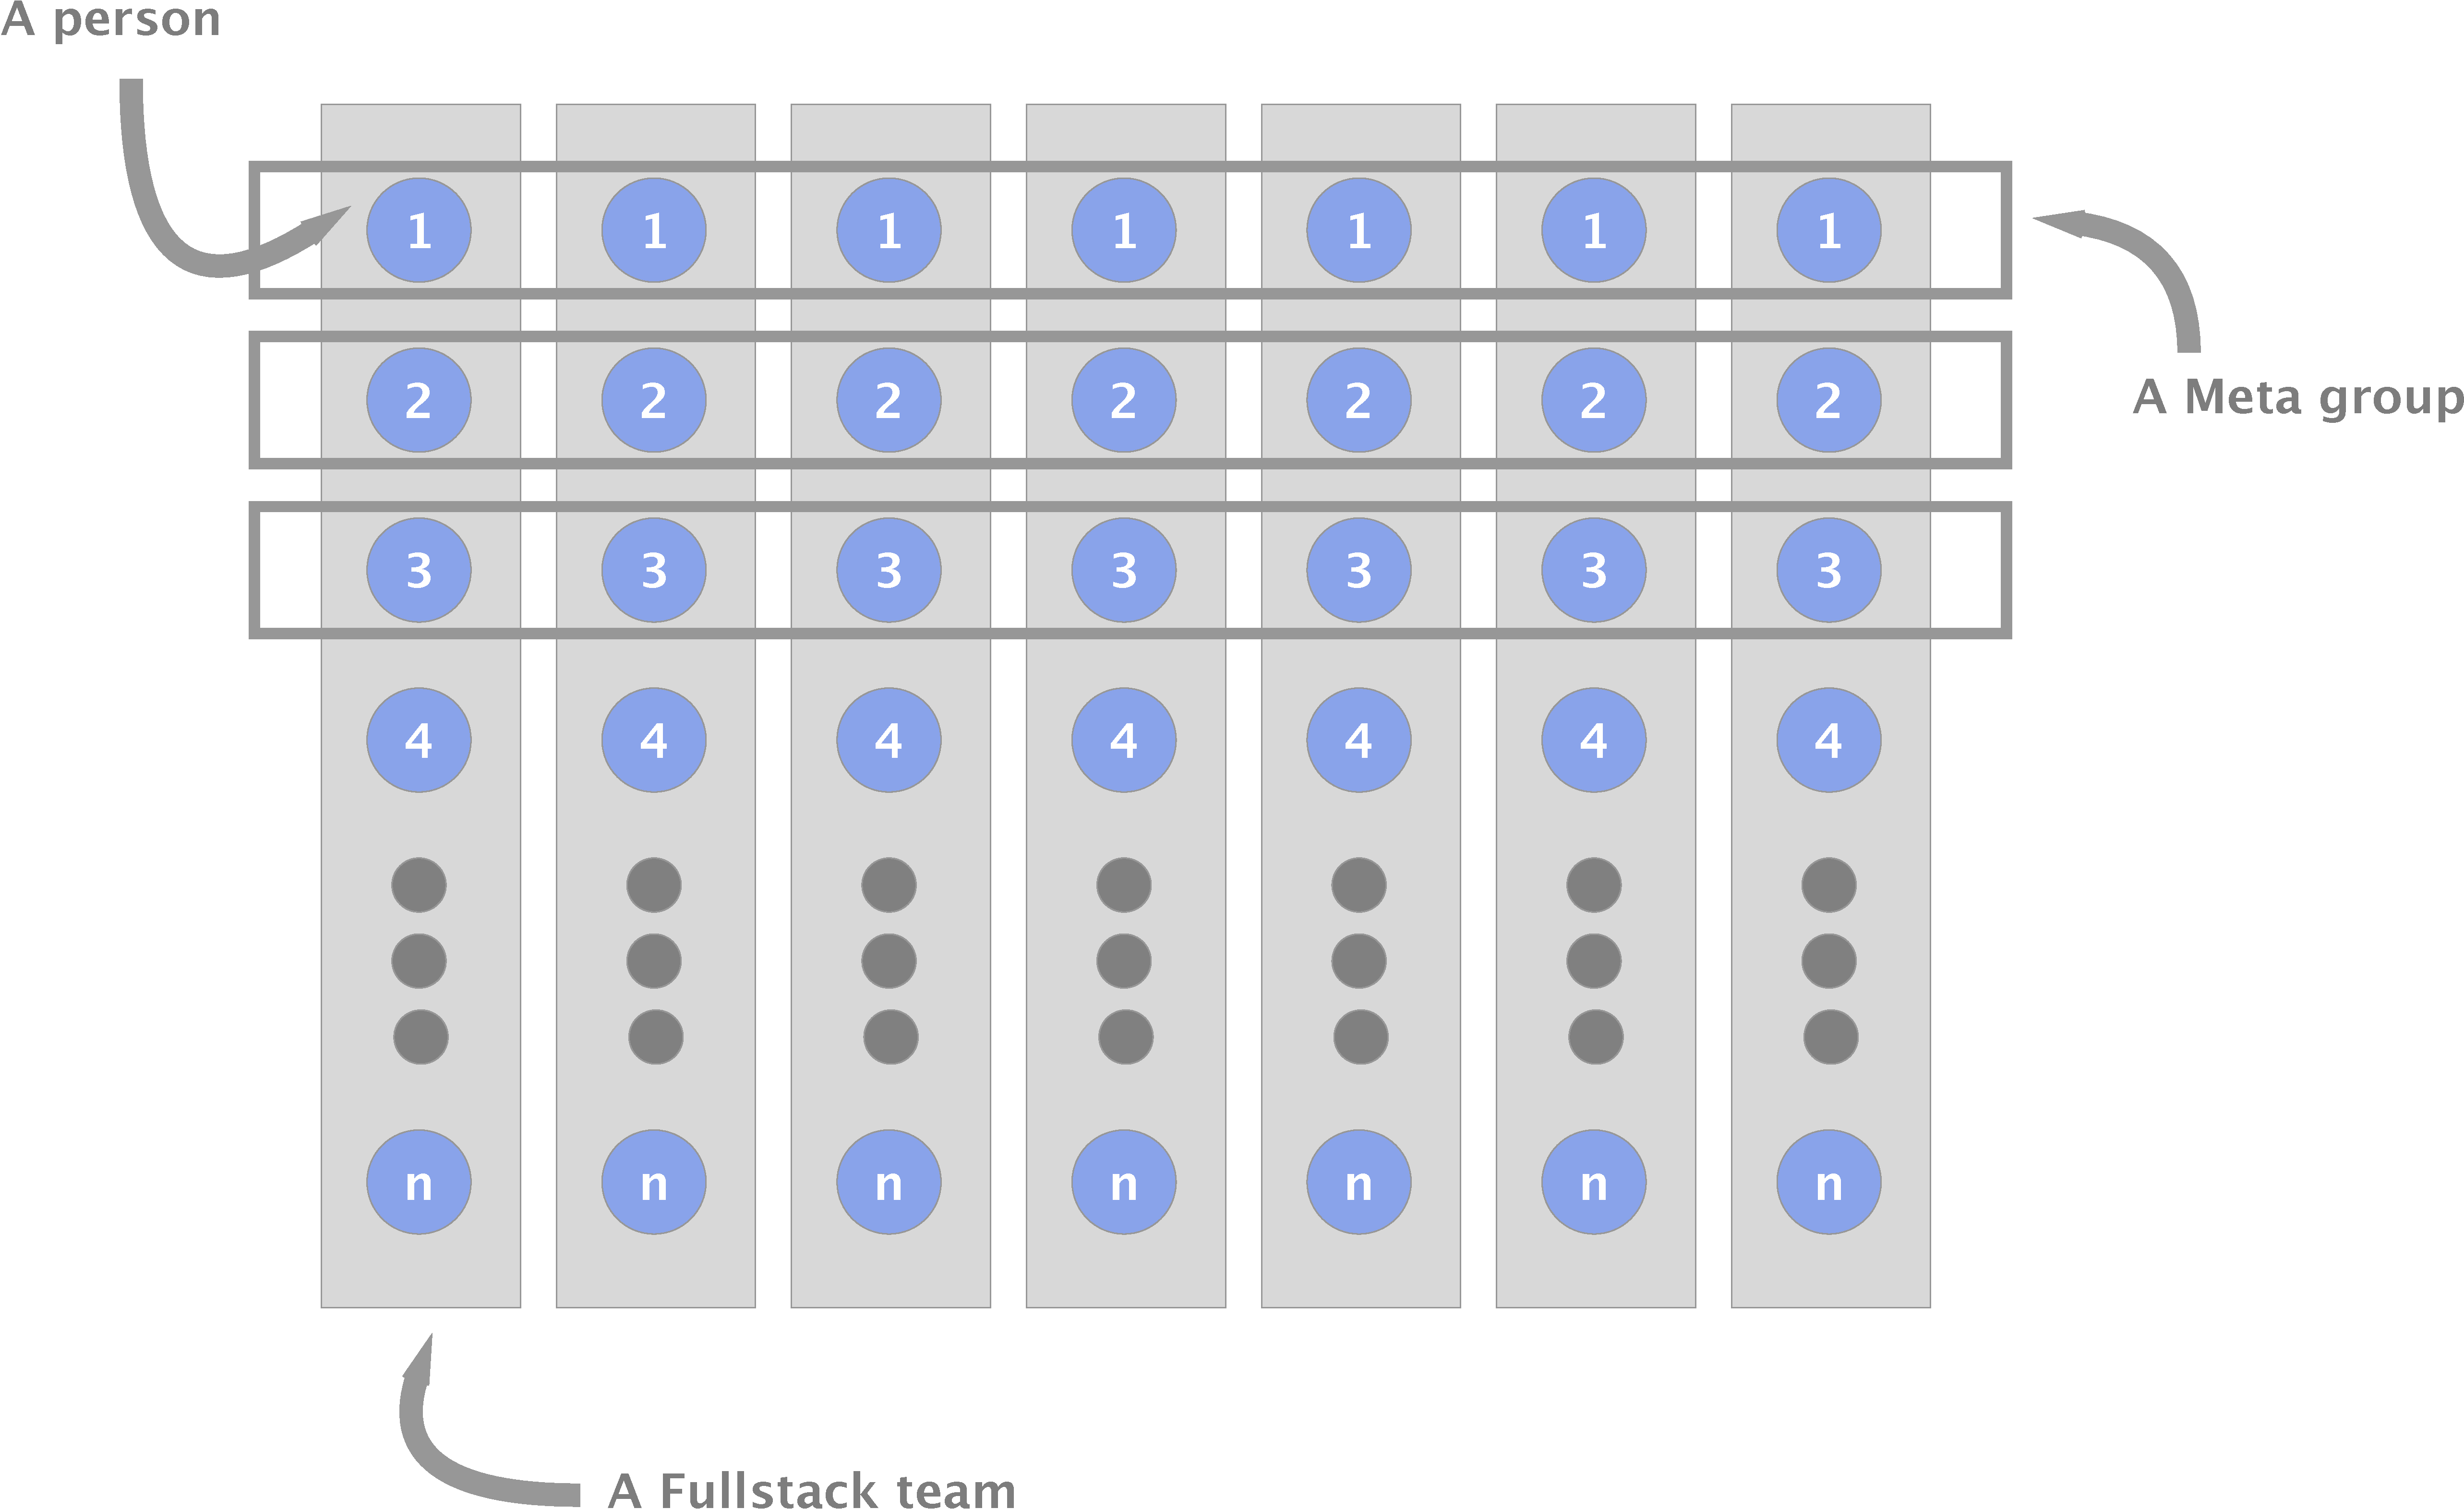
\includegraphics[width=0.95\textwidth]{figures/MetaGroupsFigure.pdf}
        \end{center}
        \caption{A illustration of how the full stack teams and meta groups are constructed}
        \label{fig:MetaGroupsFigure}
\end{figure}
\subsection{Process activities}
There are three different \glspl{skillGroup}, namely frontend, backend, and server. These groups make it possible for all \glspl{devTeam} to gain knowledge in the specific areas of the system. In the \gls{SOS} process, the activities resemble the normal scrom process where each group represents a team member in the normal Scrum process.

Using the \gls{SOS} process, we can think of each \gls{devTeam} as being a person in regular Scrum. Internally, each \gls{devTeam} has its own process. There are four sprints planned, and in the following we describe the activities that a sprint consists of:

\begin{itemize}
    \item \Gls{SOSSprintPlanning}
    \item \Gls{SOSStandUp}
    \item \Gls{skillGroup} Meetings
    \item \Gls{ReleasePreparation}
    \item \Gls{SOSSprintRetrospective}
    \item \Gls{SOSSprintReview}
    \item Release Party
\end{itemize}

\autoref{fig:SOSProcess} represents the SOS process. Placed in chronological order, each circle represents an activity, with the ones on the loop repeating. The stickmen represent a group member with a role. The "any member" role represents all of the group members. Placing a stickman in an activity means that one person from the group has to attend that activity.

One of each \gls{skillGroup} character is placed in the \gls{skillGroup} meeting activity. This means that they attend the \gls{skillGroup} meetings as representatives of their \glspl{devTeam}. If an activity does not contain a stickman, it is attended by every member of the teams.

\begin{figure}[h]
    \begin{center}
        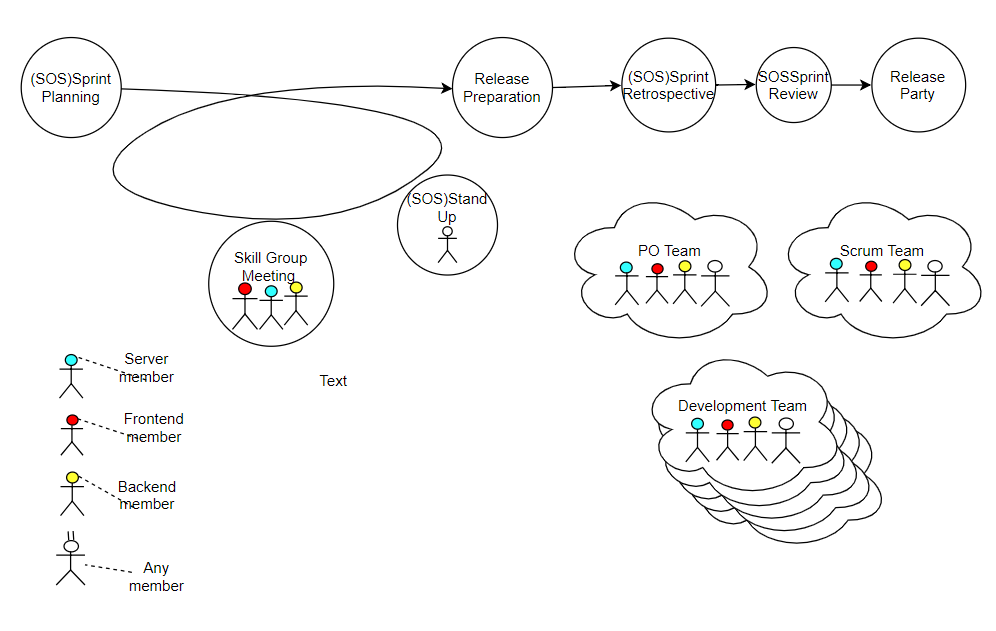
\includegraphics[width=0.95\textwidth]{figures/SOSProcess}
    \end{center}
    \caption{Representation of the \gls{SOS} process.}
    \label{fig:SOSProcess}
\end{figure}

Each cloud in the figure represents a \gls{devTeam}. \gls{SOS} only describes the process between \glspl{devTeam}. It is up to each group to define their process, as long as it fits within the \gls{SOS} guidelines.

\subsubsection{Activities}
The following part describes each of the activities.

\Gls{SOSSprintPlanning} is a meeting held on the first day of each sprint where all members of \Gls{G19} attend. Before the \Gls{SOSSprintPlanning}, the \gls{POT} has prepared user stories for the sprint backlog, and the purpose of the sprint. \gls{POT} presents these stories to the \glspl{devTeam}, and they choose which user stories they want to implement, and consensus with \gls{PO}. When the \glspl{devTeam} has found some tasks appropriate for them, they should leave the meeting. So that only groups without any tasks are present which makes it easier for the \gls{SMT} and \gls{PO} to aid them.

\Gls{SOSStandUp} is a status meeting, held one to three times a week. The purpose of this meeting is to share the progress and challenges between the teams, so the different teams know how the system is progressing and can help each other with questions. The meeting should not take more than 15 minutes.

The \Gls{skillGroup} meetings are held to ensure that the members of each \gls{skillGroup} is kept up to date with what is going on in their part of the system. The goal is to have at least one meeting every week.

\Gls{ReleasePreparation} covers four days before the end of each sprint. Here, the system is made ready for release, and the new features and changes are validated and verified.

\Gls{SOSSprintReview} is held at the end of each sprint. Here, only one group member may attend. In this meeting, each group representative talks about what that group has been working on during the sprint.

In the \gls{SOSSprintRetrospective} the development process is evaluated. Here, all group members are to participate. Before the meeting, the groups should reflect on how they feel the \gls{SOS} process has been. A small group is formed containing approximately one member from each group. The members discuss how they interpret their group's findings. This group collects the feedback of each group, and the ideas are voted on.

Finally, the Release Party. The Release Party is the last thing in each Sprint. The purpose here is to enhance the \glspl{devTeam} feeling of ownership of the GIRAF project and to enhance communication between the \glspl{devTeam}. If the different groups want to, they can present the work they have done during the Sprint.

\subsection{Practices and standards}

In the previously mentioned process manual, some standards and practices, which the \glspl{devTeam} have to follow, are mentioned. These fit into the following categories:

\begin{itemize}
    \item Coding standards
    \item Documentation standards
    \item Version control
    \item Code review
\end{itemize}

The coding standards involve naming conventions, descriptions and a few other aspects. This is done so the code is easier to read for people that need to get familiar with the system, mainly the future \glspl{devTeam}, because we found it hard to get to know the system when it was made by a lot of different people, with a lot of different coding standards.

Last year, the project and repository were moved to GitLab that takes care of the version control. At the beginning of this semester, our team moved it to Github. This is documented in \autoref{sec:GitAndCI}. The workflow of the project is done using GitFlow Workflow. The manual describes the rules for using branches. The point of the code review is to make sure that all code committed by the \glspl{devTeam} follow the coding standards. When a Team tries to merge code into production, two people from different groups have to review it. They have to go through a checklist (see \autoref{app:code-review-checklist}), to see if everything is all right.

Another decision made is, that the \glspl{devTeam} should document the implemented components, their responsibility and how it interacts with other components. This documentation should be stored in the wiki repository on the GIRAF Github page. The wiki should ultimately contain all information needed to get to know the different components in the system.

If a member of a team finds an issue in the program, he can make an issue report. This makes it possible to document errors systematically, without the \glspl{team} having to fix it themselves. If a \gls{team} however finds it important to introduce a new task to the product backlog, the team can issue a task creation request. The \gls{POT} then decides if they find it relevant to have in the product backlog.

The process between the \gls{G19} \glspl{devTeam} is defined in the manual. This process will be evaluated at each \gls{SOSSprintRetrospective}, and changed as needed. It is designed to make the collaboration between the \glspl{team} run as smoothly as possible, without interfering with the \glspl{team} internal processes.
